\documentclass{article}
\usepackage[utf8]{inputenc}
% \usepackage[english]{babel} % disabled to avoid missing language files in TinyTeX; not critical for this manuscript
\usepackage[T1]{fontenc}

% Graphics and figures
\usepackage{graphicx}
\DeclareGraphicsExtensions{.pdf,.png,.jpg}

\usepackage{caption}
\captionsetup{font=small,labelfont=bf,justification=raggedright,singlelinecheck=false, width=0.95\textwidth}

\usepackage{fancyvrb}
\usepackage{authblk}
\usepackage{hyperref}
\usepackage{pdflscape}
\usepackage{setspace}
\usepackage{lineno}
\usepackage{cite}
\usepackage{float}

% TikZ
\usepackage{tikz}
\usetikzlibrary{shapes.geometric, arrows.meta, positioning, calc, external}

% other packages
\usepackage{rotating} % for sidewaystable
\usepackage{chemformula}
\usepackage{siunitx}
\usepackage{palatino}
\usepackage{multirow}
\usepackage{dcolumn}
\usepackage{booktabs}
\usepackage{algorithmic}
\usepackage{pdfpages}
\usepackage{listings}
\usepackage{inconsolata}
\usepackage[final]{microtype} % improved kerning and line breaking

% TikZ styles for flowcharts
\tikzset{
	startstop/.style={ellipse, draw, fill=blue!10, text centered, minimum width=2.4cm, minimum height=0.9cm, font=\footnotesize},
	process/.style={rectangle, draw, fill=orange!20, text centered, minimum width=3.0cm, minimum height=0.9cm, font=\footnotesize},
	decision/.style={diamond, draw, fill=green!20, text centered, aspect=2, minimum width=2.5cm, inner sep=1pt, font=\footnotesize},
	arrow/.style={->, thick, >=stealth}
}

%----------------------------document----------------
\begin{document}
\setkeys{Gin}{width=0.99\textwidth}
%---------------------------title-------------------
	\title{Workflow-transfer benchmark of optical surface-roughness measurements against an internal tactile baseline across engineering materials and manufacturing processes}
\author{}
\vspace{-5mm}
\date{\today\\\vspace{2mm}}
\maketitle
%-------------------abstract---------------------------
\onehalfspacing
\linenumbers
\begin{abstract}
This study benchmarks exported optical roughness workflows against an internal tactile profilometry baseline across six engineering materials and multiple surface-generation processes. Rather than testing formal optical–tactile equivalence, the analysis examines which optical system–illumination workflows warrant prospective validation for specific material–process–parameter groups, and where tactile confirmation remains necessary. The main contribution is a reproducible workflow-level benchmark that integrates retrospective lowest-discrepancy, fixed-configuration, and leave-one-surface transfer analyses, thereby distinguishing local retrospective optimisation from more transferable performance.
Eight profile roughness parameters were analysed. Optical–tactile discrepancy depended strongly on workflow choice. Among the lowest-discrepancy system–illumination combinations available in the archive, the smallest median discrepancies were observed for amplitude parameters including $R_t$, $R_v$, $R_z$, and $R_{z1max}$. Exported $R_{sm}$ values required separate treatment because of scale sensitivity: multiplying retained optical $R_{sm}$ values by 1000 reduced the retrospective lowest-discrepancy median from 99.9\% to 17.3\%, although 25\% of material–process groups still exceeded 30\%.
Across strictly positive parameters, tactile random variability was generally smaller than the observed between-workflow discrepancies; the relative Type A standard uncertainty of the tactile mean had a median of 1.45\%. A fixed-configuration sensitivity analysis showed that the complete-coverage fixed workflow with the lowest median discrepancy achieved 24.8\%. In a leave-one-surface workflow-transfer check, selecting workflows from other material–process groups produced a held-out median discrepancy of 32.8\%, with 52\% of held-out groups still exceeding 30\%.
Overall, the resulting decision summaries establish a workflow-level benchmark for selecting optical candidates for prospective validation, while clearly distinguishing such candidates from claims of formal optical–tactile equivalence.

\noindent{\bf Keywords:} surface metrology; optical measurement; tactile reference; surface roughness; illumination wavelength; benchmarking; uncertainty.
\end{abstract}

\section{Introduction}\label{sec:intro}
Surface texture measurement remains central to manufacturing, where reported roughness parameters directly influence process control, specification compliance, and product traceability. In industrial practice, acceptance criteria are still commonly anchored to profile parameters such as $R_a$, $R_q$, $R_{sk}$, $R_{sm}$, $R_t$, $R_v$, $R_z$, and $R_{z1max}$. These profile-parameter labels belong to the ISO geometrical product specification framework for profile surface texture and remain distinct from a full areal-parameter assessment under ISO surface-texture terminology~\cite{ISO21920-2-2021,ISO25178-2-2021}. Tactile stylus profilometry retains practical authority as a reference workflow, despite being slower, access-limited, and potentially intrusive on delicate or highly finished surfaces.

The choice of profile rather than areal parameters in this benchmark reflects two practical constraints. First, most production tolerances, acceptance test criteria, and published interlaboratory comparisons are expressed in profile terms, so a profile-based benchmark speaks directly to current industrial metrology practice. Second, profile parameters were the only roughness-descriptor class retained consistently across all four optical instrument families in the present archive; areal parameters were either unavailable or incomparable across the heterogeneous instrument set. Extension to areal surface-texture parameters would require a separate study with harmonised areal acquisition, filtering, and parameter-calculation chains.

In manufacturing practice, different profile roughness parameters serve distinct engineering functions. $R_a$ remains the most widely used general acceptance criterion for machined surfaces and appears in most national and international surface-finish standards. $R_{z1max}$---the maximum peak-to-valley height within a sampling length---is the parameter most directly linked to functional performance in sealing, fatigue, and contact-stress applications and is commonly specified in ISO~21920-3 profile tolerancing. $R_{sm}$, the mean peak spacing, captures the periodicity and wavelength content of the texture and is relevant to lubrication, paint adhesion, and forming behaviour; however, it is also the profile parameter most sensitive to lateral sampling, filtering, and profile-element recognition algorithms, making it the most challenging descriptor in cross-instrument comparisons~\cite{ISO21920-2-2021,ISO21920-3-2021}. The present benchmark was designed to capture these functional distinctions by reporting all eight profile parameters separately rather than collapsing them into a single comparability index.

Despite decades of development, there is still no general criterion for determining when optical roughness measurements are acceptably close to tactile profile baselines across material classes and manufacturing workflows. Recent work nevertheless illustrates substantial progress in both low-force tactile/optical probing and cross-method comparison. Linz et al. presented 3D fibre probes combining tactile contact with optical read-out and very small contact force~\cite{Linz2012}. M\'inguez-Mart\'inez et al. reported an interlaboratory comparison of $R_a$ measurements made with stylus instruments and calibrated confocal microscopes~\cite{mínguezmartínez2022results-794}. Boedecker et al. discussed comparison of white-light interferometer and tactile results through transfer-characteristic control, filtering, and uncertainty contributions~\cite{Boedecker2010}. These developments expand the metrology toolbox while leaving a central comparability issue: optical and tactile systems may interrogate different effective measurands.

That comparability issue has been recognised repeatedly. Dierke and Tutsch addressed optical layer-thickness measurement of transparent materials~\cite{Dierke2012LayerThickness}. Leonhardt and Tiziani addressed optical topometry of surfaces with locally changing materials, layers, and contaminations~\cite{Leonhardt1999Topometry}. Garc\'ia et al. compared contact stylus and confocal microscopy methods from metrological and operational viewpoints~\cite{Garcia2018}. Schmidt et al. compared areal and profile methods for machined components and discussed parameter validity for different applications and materials~\cite{Schmidt2021459}. Nouira et al. described a high-precision profilometer for comparing tactile and optical probes against laser-interferometer measurements and standards~\cite{Nouira2014a}. Hoefling et al. addressed optical profilometry requirements for sheet-metal forming, including large object size, short measuring time, vertical resolution, and shining oil-covered metallic surfaces~\cite{Hoefling1999338}. Stavroulakis et al. addressed external shape measurement using artificial intelligence and optimised data fusion for industrial applications~\cite{Stavroulakis2018DataFusion}. The practical question concerns the material--process conditions under which a given optical workflow remains acceptably close to an established tactile baseline.

The physical origin of these discrepancies is also workflow-dependent. Optical roughness and topography values can be affected by the interaction between material or layer response, surface topography, spatial-frequency transfer, filtering, phase or envelope evaluation, lateral sampling, and profile-extraction choices~\cite{Dierke2012LayerThickness,Leonhardt1999Topometry,Boedecker2010,Tiziani1999324,Garcia2018}. Tactile values are instead influenced by stylus geometry, probing force, mechanical filtering by the tip, scan direction, contact accessibility, and profile specification operators~\cite{ISO3274-1996,ISO21920-3-2021,ISO16610-21-2011}. Consequently, the same exported profile parameter may represent different effective measurands unless the acquisition and processing chain is controlled explicitly.

Workflow behaviour may also vary with illumination and reconstruction strategy. Hu et al. developed a line-scanning chromatic confocal sensor for 3D profile measurement on highly reflective materials~\cite{Hu2021}. Hinz et al. compared fringe-projection systems across scale ranges and emphasised application-specific scanner selection and data evaluation in production metrology~\cite{Hinz2021}. Wang and Yang addressed saturation on highly reflective surfaces by combining adaptive and original-inverse fringe projection~\cite{Wang2023}. Schreiner et al. presented grazing-incidence infrared interferometry as a route to reduced speckle on optically rough technical surfaces~\cite{Schreiner1999115}. Tiziani et al. discussed spectral and temporal phase evaluation for interferometry and speckle applications, including optically rough surfaces~\cite{Tiziani1999324}. Sato and Ando recently proposed polynomial-exponent modelling of white-light scanning interferograms for envelope and fringe-phase identification~\cite{Sato2025486}.

Computational work places reconstruction and interpretation within the metrology chain. Xue et al. review machine-learning applications in optical metrology, including phase demodulation, unwrapping, phase-to-height conversion, intelligent sampling, noise reduction, and real-time processing~\cite{Xue2025}. Roberts et al. give industrial DUV--Vis--IR examples in which machine learning supplements traditional optical-metrology analysis models~\cite{Roberts2025}. Chen et al. use spectrum-pattern matching to reconstruct chromatic confocal surface profiles~\cite{Chen2021}. Ekberg et al. use automated boundary detection to turn OCT data into dimensional measurements of multilayer ceramic structures~\cite{Ekberg2014217}. Recent multi-task learning work also illustrates how shared models can be useful when multiple targets are learned from limited, sparse, or multi-instrument data~\cite{kucharski2025multitask-b68,Conrad2025}. Neethu and Vinod Chandra review challenges caused by imbalanced and unlabeled data in machine learning~\cite{Neethu2025}, while Pouchard et al. document reproducibility problems caused by training-data issues, platform/version differences, randomness, and hyperparameter variation in materials-informatics machine learning~\cite{Pouchard2020743}. Heterogeneous retrospective datasets also constrain the level of inference supported by such approaches.

Prior optical--tactile surface-texture comparisons can be grouped by design scope. Table~\ref{tab:lit_comparison} provides a structured summary of representative studies, organised by measurement methods, materials, parameters, and the type of comparability reported.

\begin{table}[H]
\centering
\small
\caption{Structured summary of representative optical--tactile surface-texture comparison studies.}
\label{tab:lit_comparison}
\setlength\tabcolsep{3.5pt}
\resizebox{\linewidth}{!}{%
\begin{tabular}{p{2.6cm} p{1.8cm} p{1.6cm} p{2.4cm} p{2.4cm} p{2.0cm}}
\toprule
Study & Materials & Parameters & Methods compared & Key finding & Gap \\
\midrule
M\'inguez-Mart\'inez et al.~\cite{mínguezmartínez2022results-794} & Metallic roughness standard & $R_a$ & Stylus vs.\ confocal microscope (interlaboratory) & Calibrated confocal comparable with stylus for $R_a$ & Single parameter, single material class \\
\midrule
Garc\'ia et al.~\cite{Garcia2018} & General engineering surfaces & Surface texture & Stylus vs.\ confocal (metrological \& operational) & Stylus most reliable; confocal offers higher resolution & No multi-material ranking or fixed-workflow analysis \\
\midrule
Schmidt et al.~\cite{Schmidt2021459} & Machined components & Profile \& areal & Tactile vs.\ stripe-light projection & Parameter validity depends on application and material & No workflow-transfer assessment \\
\midrule
Boedecker et al.~\cite{Boedecker2010} & Shape standards & Shape/topography & White-light interferometer vs.\ tactile & Comparability requires spatial-frequency transfer control and filtering & Focus on shape, not production roughness parameters \\
\midrule
Nouira et al.~\cite{Nouira2014a} & V-groove \& aspherical standards & Form, roughness & High-precision profilometer: tactile vs.\ confocal chromatic & Nanometric comparison of probe linear residuals & Standards, not production surfaces \\
\midrule
Hoefling et al.~\cite{Hoefling1999338} & Sheet-metal (car body) & Form, surface texture & Fringe projection vs.\ tactile & Object size, reflectivity, and cycle time constrain optical use & Application-specific, single optical technique \\
\midrule
Marichamy et al.~\cite{Marichamy2025} & L-PBF $\alpha$-Ti-6Al-4V & Hole quality, $R_a$, $R_z$ & Optical profilometry vs.\ tactile & Process-parameter effects on surface finish for orthopaedic implants & Single material, single manufacturing route \\
\midrule
Hu et al.~\cite{Hu2021} & Highly reflective materials & 3D profile & Line-scanning chromatic confocal sensor & Sensor design validated for reflective surfaces & Instrument-development focus, no tactile baseline \\
\midrule
\textbf{This work} & \textbf{6 materials, 9 processes} & \textbf{8 profile parameters} & \textbf{4 optical families vs.\ tactile} & \textbf{Three-view benchmark: local selection, fixed workflow, held-out transfer} & --- \\
\bottomrule
\end{tabular}
}
\end{table}

What these studies share is a reporting pattern in which best-case or per-condition comparability is discussed, but the penalty associated with fixing one optical configuration before measurement, or transferring a workflow choice from one material class to another, is rarely quantified. No prior study has, to our knowledge, combined the three operational views---local retrospective selection, fixed single-configuration sensitivity, and held-out surface-class transfer---within a single, reproducible, multi-material, multi-parameter benchmarking framework.

Existing optical--tactile comparisons often report comparability for selected instruments, surfaces, or parameters, but they rarely separate three operational questions that a practitioner must answer when integrating optical roughness measurement into a quality-control workflow: (i)~whether a low-discrepancy optical candidate exists locally for a specific material--process combination, (ii)~what penalty is incurred when one optical configuration must be fixed before measurement across a broad and heterogeneous surface range, and (iii)~whether workflow choices that perform well on known surface classes transfer reliably to previously unseen material--process classes. This distinction matters because industrial laboratories rarely have the freedom to select a different optical instrument for each parameter--surface group. The present benchmark addresses this gap by designing the comparison space around these three views and by making the selection penalty quantitatively visible. The intended practical output is a set of decision tables and discrepancy maps that allow a metrology laboratory to identify which parameter--material--process combinations are the most promising candidates for prospective, protocol-driven validation and which combinations should remain with tactile measurement until a dedicated optical validation study is performed.

The contribution is a structured, reproducible benchmark of workflow discrepancy within the analysed archive. Its novelty is the combination of three complementary views of optical workflow performance: local lowest-discrepancy selection, fixed-configuration sensitivity, and held-out surface-class transfer. This design makes the optimisation effect visible instead of reporting only the most favourable optical--tactile matches. The comparison space is defined by matched exported parameter labels and is used to characterise workflow-level discrepancy patterns for follow-up validation.

\section{Methods}

\subsection{Study design and unit of analysis}
This work presents a retrospective benchmark based on an archived dataset of tactile and optical measurements acquired across six engineering materials and multiple surface-generation routes. Each observation is defined by specimen identity, roughness parameter, optical system, illumination condition, optical output, and the corresponding tactile result. The primary unit of comparison is the parameter–surface group, defined as a single roughness parameter within a given material–process combination.
Within the manuscript subset, each of the eight parameters contributes 59 material–process groups, giving a total of 472 parameter–surface groups. Because not every optical workflow is represented in every group, all analyses were conducted on the available comparable subset for each task.

Archive specimen labels follow the pattern \texttt{<material>\_<process>} (for example, \texttt{ti6al4v\_mf} or \texttt{14301\_wedm\_f}). Material identifiers denote C45 steel (\texttt{c45}), AISI~304 stainless steel / EN~1.4301 (\texttt{14301}), Ti6Al4V (\texttt{ti6al4v}), Al7075 (\texttt{al7075}), MO58A brass (\texttt{mo58a}), and ELLOR graphite (\texttt{ellor}). Process identifiers denote rough milling (\texttt{mr}), finish milling (\texttt{mf}), rough and finish face turning (\texttt{tr}, \texttt{tf}), burnishing after finish milling (\texttt{b}), rough and finish wire electrical discharge machining (\texttt{wedm\_r}, \texttt{wedm\_f}), grinding (\texttt{gri}), glass bead blasting (\texttt{gla}), and honing (\texttt{hon}). The manuscript tables expand these archive codes for readability, whereas the exported archive files retain the short slugs.

The process labels denote archived surface-generation route classes rather than complete manufacturing recipes. Detailed process metadata—including tool geometry, feed and speed settings, depths of cut, wire EDM discharge settings, and abrasive or honing conditions—were retained unevenly across materials. Accordingly, material–process groups were analysed as benchmark strata rather than as factors in a designed manufacturing experiment.

\subsection{Tactile baseline}
Tactile stylus profilometry was treated as the internal baseline because it was the only workflow in the archive for which repeated measurements were retained consistently across the manuscript subset. The terminology for measurement uncertainty follows VIM and GUM usage, distinguishing repeatability descriptors from a traceability-qualified uncertainty budget~\cite{JCGM200-2012,JCGM100-2008}. For each specimen and roughness parameter, the tactile mean
\[
S=\frac{1}{n_S}\sum_{k=1}^{n_S}T_k
\]
was computed from $n_S=20$ repeats, with accompanying repeatability standard deviation $s_S$ and Type A standard uncertainty of the mean $u_S=s_S/\sqrt{n_S}$. These quantities describe internal repeatability and the Type A component available from the archive; they are reported separately from traceability-qualified uncertainty.

The tactile mean was therefore used as an internal baseline rather than as a fully traceability-qualified reference value. Although the retained archive supports Type A repeatability descriptors for tactile measurements, it does not provide a complete combined uncertainty budget incorporating stylus geometry, probing force, calibration artefact uncertainty, filtering choices, optical vertical and lateral calibration, optical repeatability, and reconstruction settings. Prospective validation would additionally require documented contact-instrument characteristics and profile specification operators, including stylus geometry, nominal contact conditions, evaluation length, and profile assessment rules consistent with profile GPS standards~\cite{ISO3274-1996,ISO21920-3-2021}. Consequently, the reported values quantify exported-workflow discrepancy within the archive and should be interpreted as screening evidence for prospective validation.

\subsection{Optical workflows and comparison space}
The optical archive includes confocal microscopy, focus variation, confocal--interferometric fusion, and interferometry-based systems, with multiple illumination bands where available. System abbreviations used in the figures and tables follow the archive nomenclature: \emph{conf} for confocal microscopy, \emph{FV} for focus variation, \emph{fusion} for confocal--interferometric fusion, and \emph{int} for interferometry/coherence-scanning interferometry.

Comparison was restricted to matched specimen identity and same-named exported roughness parameters. The retained optical metadata identify workflow family and illumination condition; retained row labels also encode nominal x10 and 5x5 acquisition labels, but not enough numerical information to reconstruct objective, sampling, filtering, form-removal, or reconstruction settings across all instruments. The retained values are instrument-exported profile-parameter labels rather than raw areal maps or reconstructed profile traces, so profile direction, profile averaging, lateral resampling, and profile-extraction settings cannot be harmonised uniformly. A prospective raw-profile comparison would require a common filtering and form-removal chain, including ISO/GPS profile-filter choices~\cite{ISO16610-21-2011}. The reported discrepancies are between-workflow discrepancies within this exported-parameter comparison space.

\begin{table}[H]
\centering
\small
\caption{Retained archive fields and metrological role in the workflow benchmark}
\label{tab:retained_metadata}
\setlength\tabcolsep{4pt}
\resizebox{\linewidth}{!}{%
\begin{tabular}{lll}
\toprule
Information element & Retention in archive & Role in the present analysis \\
\midrule
Material, process, and specimen identifiers & Retained & Define material--process strata and matched comparison groups \\
Profile roughness parameter labels & Retained & Define same-named exported-parameter comparisons \\
Tactile repeats & Retained consistently ($n_S=20$) & Internal baseline mean and repeatability descriptor \\
Optical workflow family and illumination condition & Retained & System+illumination ranking, fixed-workflow analysis, transfer check \\
Optical exported roughness output & Retained & Optical--tactile discrepancy calculation \\
Nominal acquisition labels & Partially retained & Qualitative archive metadata; not sufficient for full reconstruction \\
Raw tactile/optical profiles and areal maps & Not retained uniformly & Excluded from common raw-profile measurand reconstruction \\
Filtering, form removal, and profile-extraction settings & Not retained uniformly & Treated as part of the workflow-level comparison frame \\
Optical objective, sampling, resolution, and calibration metadata & Not retained uniformly & Discussed as prospective-validation requirements \\
Combined tactile--optical uncertainty budget & Not retained & Outside the retrospective benchmark scope \\
\bottomrule
\end{tabular}
}
\end{table}

\subsection{Response variables}
The parameter symbols follow the profile roughness notation used in ISO surface-texture terminology. The comparison is restricted to same-named exported profile parameters; areal surface-texture parameters were outside the retained manuscript subset. For the seven strictly positive roughness parameters ($R_a$, $R_q$, $R_{sm}$, $R_t$, $R_v$, $R_z$, and $R_{z1max}$), discrepancy between optical output $O$ and tactile baseline $S$ was defined as
\begin{equation}
d_p = 100\left|\frac{O-S}{S}\right|.
\label{eq:diff}
\end{equation}
For the sign-sensitive parameter $R_{sk}$, near-zero tactile denominators make percentage normalisation unstable. Archive-derived decision or regression summaries that retain percentage-based $R_{sk}$ values are treated as secondary screening descriptors, separately from the strictly positive parameters.

\subsection{Decision-oriented summaries}
Within each parameter--surface group, optical workflows were ranked by the available observed discrepancy, using the median when more than one retained optical output was available for the same system--illumination pair. In the archived decision subset, optical replication is incomplete; most system--illumination entries represent one exported optical result matched to a tactile mean. The decision tables report the minimum retained discrepancy across the tested system--illumination combinations and identify the workflow that achieved it. These retrospective summaries describe lowest-discrepancy behaviour within the archive, separately from the performance expected for a single fixed optical configuration.

To quantify this optimisation effect, a fixed-configuration sensitivity analysis was performed for the seven strictly positive parameters. Each candidate optical workflow was defined as one system--illumination pair and was evaluated across all parameter--surface groups in which that pair was available, without allowing the workflow to vary by group. The resulting fixed-workflow medians were compared with the retrospective lowest-discrepancy medians from the same groups. Coverage was reported relative to the 413 strictly positive parameter--surface groups used in the decision summaries.

A leave-one-surface workflow-transfer check was then performed to estimate how well workflow choices selected from the archive transfer to a held-out surface class. For each strictly positive parameter and held-out material--process group, system--illumination workflows were ranked using all other material--process groups for the same parameter. The highest-ranked workflow available for the held-out group was then evaluated on that held-out group. This analysis remains retrospective and archive-based, but the held-out group is not used to rank candidate workflows.

The retained metadata are summarised in Table~\ref{tab:retained_metadata}. Accordingly, the release supports a retrospective workflow benchmark rather than a prospective traceability-oriented validation study.

All numerical summaries reported in the manuscript and supplement were generated automatically by documented Python scripts (\texttt{generate\_supplement.py} and the analysis modules in the public repository) from the same archived CSV output files distributed in the reproducibility package. Manual calculation steps are limited to cross-checking the manuscript table entries against the archived CSVs and verifying that the decision-table logic matches the documented ranking rules. A data dictionary mapping each CSV column to its definition, units, and source is included in the repository \texttt{README} and in the supplement. Independent verification of the reported results is possible without access to raw instrument files: the public CSV outputs can be downloaded, the supplied Python scripts executed, and the generated tables and figures compared against those in the manuscript and supplement.

The 10\% and 30\% discrepancy bands used in the decision summaries are operational triage bands, not tolerance limits, conformance criteria, or substitutes for application-specific measurement uncertainty statements. The 10\% threshold approximates the typical calibration-grade agreement expected between two instruments of the same type measuring the same roughness parameter and corresponds loosely to the expanded uncertainty routinely reported in accredited dimensional calibration laboratories. The 30\% threshold identifies parameter--surface groups where the optical--tactile discrepancy exceeds a level that most industrial quality-control applications would accept without further investigation. These bands are pragmatic screening tools derived from inspection of the archive-level discrepancy distributions and are not derived from formal tolerance-grade standards such as ISO~21920-3; their relationship to ISO tolerance grades is discussed in Section~\ref{sec:discussion}.

\subsection{Statistical analysis}
Statistical analyses were performed within parameter--surface groups. Two-factor ANOVA with factors \emph{system} and \emph{illumination colour} provided an exploratory decomposition of variance. In this retrospective, unbalanced archive, nominal $p$-values served as screening statistics; no family-wise confirmatory inference was claimed across the large number of per-group screens. Interpretation was based primarily on effect sizes and on consistency of patterns across groups.

System-wise linear regressions of discrepancy versus nominal illumination wavelength were used as low-degree-of-freedom descriptive summaries. Most fits rely on three or four wavelength levels and were treated as screening trends rather than physical calibration laws.

Non-parametric percentile bootstrap intervals were computed for the aggregate retrospective lowest-discrepancy medians by parameter, material, and process. Bootstrap resampling was performed across archive-defined parameter--surface groups within each aggregate stratum, using 2000 resamples and a fixed random seed; these intervals describe stability of the retrospective median summaries and are not prospective validation intervals.

Supplementary tables and representative figures were generated from the same exported analysis outputs used in the main manuscript. The supplement generator (\texttt{generate\_supplement.py}) formats the ANOVA screens, wavelength-regression summaries, system descriptives, tactile repeatability summaries, bootstrap stability summaries, and selected representative figures without adding a separate statistical model.

To compare workflow similarity within a given parameter--surface group, a technical distance matrix was defined from mean discrepancies. If $\bar d_i$ and $\bar d_j$ denote mean discrepancy for techniques $i$ and $j$, where a technique is one optical system under one illumination condition, then
\begin{equation}
D_{ij}=|\bar d_i-\bar d_j|.
\label{eq:distance}
\end{equation}
This quantity describes similarity of discrepancy patterns within the analysed dataset, separately from traceability, matched calibration, or measurand equivalence.

\section{Results}

Across the manuscript subset, each of the eight parameters contributes 59 material--process groups, yielding 472 parameter--surface groups overall, all with tactile baselines based on $n_S=20$ repeats. For the seven strictly positive parameters, the relative Type A standard uncertainty of the tactile mean had median 1.45\% and interquartile range 0.85--2.44\%; parameter-wise summaries are reported in Supplementary Table~S4. The random variability of tactile measurements is generally smaller than the between-workflow discrepancies analysed below, supporting the use of the tactile mean as an internal benchmark baseline.

\subsection{Decision-oriented benchmark summaries}
For each parameter--surface group, the decision summaries retain the lowest observed median discrepancy across the tested system and illumination combinations. These tables describe retrospective lowest-discrepancy performance within the archive, separately from the behaviour of any single fixed configuration.

Table~\ref{tab:decision_by_param} summarises retrospective lowest-discrepancy medians for the seven strictly positive parameters. Among them, amplitude-type measures ($R_t$, $R_v$, $R_z$, and $R_{z1max}$) achieve the lowest medians, ranging from 4.8\% to 6.6\%; $R_a$ and $R_q$ remain below 10\% in median terms, whereas $R_{sm}$ remains problematic at 99.9\%. No single optical workflow dominates all parameters, although interferometry-based configurations are frequently among the lowest-discrepancy options. Percentage-based $R_{sk}$ rankings are excluded from the manuscript decision tables due to near-zero tactile denominator instability; they are retained as archive-level screening outputs.

The band columns in Table~\ref{tab:decision_by_param} provide a practical triage view rather than a normative acceptance rule. Groups in the lowest band identify candidate optical workflows for prospective protocol validation, groups in the middle band indicate cases where material--process-specific checking remains important, and groups above 30\% describe conditions where tactile confirmation or a revised optical protocol remains the more defensible route. The same interpretation separates $R_{sm}$ from the amplitude parameters: all 59 $R_{sm}$ groups remain in the high-discrepancy band, whereas the lower-discrepancy band contains 63--69\% of the $R_t$, $R_v$, $R_z$, and $R_{z1max}$ groups.

% Auto-generated by make_results_decision_tables.R
\begin{table}[H]
\centering
\small
\caption{Decision-oriented summary of optical--tactile discrepancy by strictly positive roughness parameter (lowest-discrepancy system+colour chosen per material--process group)}
\label{tab:decision_by_param}
\setlength\tabcolsep{4pt}
\resizebox{\linewidth}{!}{%
\begin{tabular}{lccccccc}
\toprule
Parameter & $N$ & Lowest median $|\mathrm{diff}|$ [\%] & Q1--Q3 & $\leq 10\%$ & 10--30\% & >30\% & Most frequent lowest (system, colour) \\
\midrule
$R_a$ & 59 & 9.8 & 2.6--21.8 & 30 (51\%) & 16 (27\%) & 13 (22\%) & int, red \\
$R_q$ & 59 & 7.4 & 2.4--22.5 & 35 (59\%) & 12 (20\%) & 12 (20\%) & int, red \\
$R_{sm}$ & 59 & 99.9 & 99.9--99.9 & 0 (0\%) & 0 (0\%) & 59 (100\%) & int, white \\
$R_t$ & 59 & 6.6 & 2.1--13.2 & 39 (66\%) & 13 (22\%) & 7 (12\%) & int, green \\
$R_v$ & 59 & 4.8 & 1.3--19.0 & 40 (68\%) & 7 (12\%) & 12 (20\%) & int, red \\
$R_z$ & 59 & 5.3 & 1.2--20.3 & 37 (63\%) & 10 (17\%) & 12 (20\%) & int, red \\
$R_{z1max}$ & 59 & 5.7 & 2.0--12.3 & 41 (69\%) & 10 (17\%) & 8 (14\%) & int, red \\
\bottomrule
\end{tabular}
}
\vspace{0.5ex}
\begin{minipage}{\linewidth}
\footnotesize\textit{Note:} $N$ is the number of available material--process groups for the seven strictly positive parameters. For each group, the optical configuration (system+illumination colour) that minimises the median $|\mathrm{diff}|(\%)$ is selected. Q1--Q3 are quartiles of the selected medians. The band columns ($\leq 10\%$, 10--30\%, >30\%) count how many groups fall into each range; values are shown as count (percent of $N$), e.g. 7 (15\%) means 7 groups, i.e. 15\% of $N$. Most frequent lowest denotes the modal selected (system, colour) across groups. Percentage-based $R_{sk}$ rankings are excluded from the manuscript decision tables because normalisation becomes unstable near zero; archive-level screening rows are retained separately in the exported outputs.
\end{minipage}
\end{table}


Because $R_{sm}$ was the only strictly positive parameter that remained uniformly in the high-discrepancy band, it was segmented separately by optical system, material, and process (Table~\ref{tab:rsm_diagnostic}). The diagnostic segmentation shows that the effect is not concentrated in one workflow family or one surface class. For all four optical-system families, every retained $R_{sm}$ system--colour entry exceeded 30\% discrepancy. After retrospective lowest-discrepancy workflow selection, every material stratum and every process stratum also remained entirely above 30\% discrepancy.

% Auto-generated by make_results_decision_tables.R
\begin{table}[H]
\centering
\small
\caption{Diagnostic segmentation of $R_{sm}$ optical--tactile discrepancy by optical system, material, and process}
\label{tab:rsm_diagnostic}
\setlength\tabcolsep{4pt}
\resizebox{\linewidth}{!}{%
\begin{tabular}{llcccccc}
\toprule
View & Stratum & $N$ & Median $|\mathrm{diff}|$ [\%] & Q1--Q3 & $\leq 10\%$ & >30\% & Modal workflow \\
\midrule
Optical system & conf & 172 & 100.0 & 99.9--100.0 & 0 (0\%) & 172 (100\%) & all colours \\
Optical system & FV & 177 & 99.9 & 99.9--99.9 & 0 (0\%) & 177 (100\%) & all colours \\
Optical system & fusion & 177 & 100.0 & 100.0--100.0 & 0 (0\%) & 177 (100\%) & all colours \\
Optical system & int & 233 & 99.9 & 99.9--99.9 & 0 (0\%) & 233 (100\%) & all colours \\
\addlinespace
Material & AISI 304 / EN 1.4301 (14301) & 10 & 99.9 & 99.9--99.9 & 0 (0\%) & 10 (100\%) & FV, white \\
Material & Al7075 & 10 & 99.9 & 99.8--99.9 & 0 (0\%) & 10 (100\%) & FV, white \\
Material & C45 steel & 10 & 99.9 & 99.9--99.9 & 0 (0\%) & 10 (100\%) & int, white \\
Material & Graphite (ELLOR) & 9 & 99.9 & 99.9--99.9 & 0 (0\%) & 9 (100\%) & int, blue \\
Material & MO58A brass & 10 & 99.9 & 99.9--99.9 & 0 (0\%) & 10 (100\%) & FV, green \\
Material & Ti6Al4V & 10 & 99.9 & 99.9--99.9 & 0 (0\%) & 10 (100\%) & int, white \\
\addlinespace
Process & MR (rough milling) & 6 & 99.9 & 99.8--99.9 & 0 (0\%) & 6 (100\%) & int, white \\
Process & MF (finish milling) & 6 & 99.9 & 99.9--100.0 & 0 (0\%) & 6 (100\%) & int, white \\
Process & TR (rough face turning) & 6 & 99.8 & 99.7--99.8 & 0 (0\%) & 6 (100\%) & int, white \\
Process & TF (finish face turning) & 6 & 99.8 & 99.6--99.9 & 0 (0\%) & 6 (100\%) & int, white \\
Process & B (burnishing after MF) & 5 & 99.9 & 99.9--100.0 & 0 (0\%) & 5 (100\%) & int, white \\
Process & WEDM\_R (rough wire EDM) & 6 & 99.9 & 99.9--99.9 & 0 (0\%) & 6 (100\%) & int, blue \\
Process & WEDM\_F (finish wire EDM) & 6 & 99.9 & 99.9--99.9 & 0 (0\%) & 6 (100\%) & FV, green \\
Process & GRI (grinding) & 6 & 99.9 & 99.9--99.9 & 0 (0\%) & 6 (100\%) & FV, green \\
Process & GLA (glass bead blasting) & 6 & 99.9 & 99.9--99.9 & 0 (0\%) & 6 (100\%) & FV, green \\
Process & HON (honing) & 6 & 99.9 & 99.9--99.9 & 0 (0\%) & 6 (100\%) & FV, green \\
\bottomrule
\end{tabular}
}
\vspace{0.5ex}
\begin{minipage}{\linewidth}
\footnotesize\textit{Note:} Optical-system rows summarise all retained $R_{sm}$ system--colour entries. Material and process rows summarise the retrospective best-achievable $R_{sm}$ discrepancy per material--process group. The modal workflow is the most frequently selected best system+colour within the corresponding material or process stratum; for optical-system rows, all retained illumination colours are pooled.
\end{minipage}
\end{table}


The retained $R_{sm}$ comparison was then examined for unit-scale sensitivity because optical spacing exports were numerically much smaller than the tactile spacing values. Multiplying optical $R_{sm}$ values by 1000, treated as a post hoc millimetre-to-micrometre sensitivity rather than as a primary correction, reduced the all-entry median discrepancy from 99.9\% to 47.4\% and the lowest-discrepancy workflow median across material--process groups from 99.9\% to 17.3\% (Table~\ref{tab:rsm_scale_sensitivity}). Under this sensitivity, 24 of 59 lowest-discrepancy workflow groups moved into the $\leq 10\%$ band, while 15 of 59 remained above 30\%. Accordingly, retained exported-value $R_{sm}$ is not used to support practical optical-substitution recommendations; it is retained as a harmonisation-sensitive diagnostic pending raw-profile validation.

% Auto-generated by make_results_decision_tables.R
\begin{table}[H]
\centering
\small
\caption{Sensitivity of $R_{sm}$ discrepancy to retained optical unit scale}
\label{tab:rsm_scale_sensitivity}
\setlength\tabcolsep{4pt}
\resizebox{\linewidth}{!}{%
\begin{tabular}{llcccccc}
\toprule
Comparison set & Scale assumption & $N$ & Median $|\mathrm{diff}|$ [\%] & Q1--Q3 & $\leq 10\%$ & >30\% & Median tactile/optical ratio \\
\midrule
All retained system-colour entries & Exported optical value & 761 & 99.9 & 99.9--100.0 & 0 (0\%) & 761 (100\%) & 1799.8 \\
All retained system-colour entries & Optical value multiplied by 1000 & 761 & 47.4 & 28.0--66.0 & 53 (7\%) & 558 (73\%) & 1.8 \\
\addlinespace
Lowest-discrepancy workflow per material-process group & Exported optical value & 59 & 99.9 & 99.9--99.9 & 0 (0\%) & 59 (100\%) & 1030.4 \\
Lowest-discrepancy workflow per material-process group & Optical value multiplied by 1000 & 59 & 17.3 & 3.9--30.2 & 24 (41\%) & 15 (25\%) & 1.2 \\
\bottomrule
\end{tabular}
}
\vspace{0.5ex}
\begin{minipage}{\linewidth}
\footnotesize\textit{Note:} The x1000 rows are a sensitivity check that treats retained optical $R_{sm}$ values as if they were exported in millimetres and converted to micrometres before comparison. They are not used as corrected primary endpoints because complete original unit metadata and raw processing chains are not retained consistently across the archive.
\end{minipage}
\end{table}


Tables~\ref{tab:decision_by_process} and~\ref{tab:decision_by_material} aggregate the same retrospective lowest-discrepancy summaries by surface-generation process and by material across the 413 strictly positive parameter--surface groups. Even after allowing the system and illumination to vary, process and material still strongly modulate how often optical workflows enter a low-discrepancy regime.

The best-agreement and worst-agreement material--process strata can be identified directly from these tables. Finish wire-EDM C45 steel and ground C45 steel consistently showed the lowest retrospective amplitude-parameter discrepancies, with $R_t$, $R_v$, $R_z$, and $R_{z1max}$ medians below 5\% after workflow selection. Honed MO58A brass and glass-bead-blasted 14301 stainless steel also occupied favourable positions across most amplitude parameters. At the opposite end, rough face-turned Ti6Al4V and ELLOR graphite, together with rough-milled 14301 stainless steel, repeatedly occupied the highest-discrepancy cells. Ti6Al4V surfaces combine moderate reflectance with a directional, anisotropic milled or turned texture that interacts strongly with the optical footprint and illumination geometry; the material's optical constants ($n \approx 3.4$, $k \approx 4.2$ at visible wavelengths) indicate higher absorption than typical engineering steels, which can reduce the signal-to-noise ratio in confocal and interferometric measurements. Rough-milled 14301 stainless steel ($n \approx 2.5$, $k \approx 3.5$ at 633~nm) presents a different challenge: its high reflectance and the steep local slopes in the milled texture can exceed the acceptance angle of confocal objectives, causing data dropout and reconstruction artefacts that inflate the exported roughness values. ELLOR graphite presents low reflectance, high porosity, and subsurface scattering that challenge most optical profiling principles. 

As a concrete worst-case illustration, the rough-face-turned Ti6Al4V group (\texttt{ti6al4v\_tf}) is examined in detail using the same analytical structure applied to the best-case groups throughout Section~3. Under retrospective lowest-discrepancy selection, all amplitude parameters for this group fall into the 10--30\% middle band, and $R_{sm}$ remains above 99.9\%. When the workflow is fixed to the lowest-median complete-coverage configuration (interferometry with green illumination), the discrepancy moves several amplitude parameters from the middle band into the $>$30\% band, consistent with the overall fixed-workflow median of 24.8\% (Table~\ref{tab:fixed_workflow_sensitivity}). Under leave-one-surface transfer, the held-out discrepancy for this group places it among the 52\% of parameter--surface groups that remain above 30\% (Table~\ref{tab:workflow_transfer}). The technical distance matrix for this group (Supplementary Figure for \texttt{ti6al4v\_tf}) shows that the four optical families separate into two clusters differing by more than 20 percentage points in mean discrepancy, confirming that the choice of optical system---not just the material---is decisive even in unfavourable conditions. The practical consequence is that Ti6Al4V, 14301 stainless steel in rough-milled condition, and ELLOR graphite should remain with tactile measurement until a dedicated, a priori designed prospective validation study demonstrates workflow-specific agreement below the relevant application tolerance. The full per-parameter decision tables, effect-size decompositions, wavelength regressions, and technical distance maps for every material--process group are provided in the supplementary material, allowing the reader to conduct the same worst-case--best-case comparison for any group of interest.

The extreme-case identifications serve as screening flags for follow-up investigation rather than as statements about material--process suitability for optical measurement in general.

Bootstrap percentile intervals for the aggregate medians are reported in Supplementary Table~S5. They support the same hierarchy as the point estimates: amplitude-parameter medians remain in the lower-discrepancy range, retained exported-value $R_{sm}$ remains close to 100\%, and process-level intervals are wider where the archive combines more heterogeneous surface-generation routes.

% Auto-generated by make_results_decision_tables.R
\begin{table}[H]
\centering
\small
\caption{Decision summary aggregated by surface-generation process across all materials and strictly positive parameters}
\label{tab:decision_by_process}
\setlength\tabcolsep{4pt}
\resizebox{\linewidth}{!}{%
\begin{tabular}{lccccccc}
\toprule
Process & $N$ & Median best $|\mathrm{diff}|$ [\%] & Q1--Q3 & $\leq 10\%$ & 10--30\% & >30\% & Most frequent best (system, colour) \\
\midrule
GLA (glass bead blasting) & 42 & 4.7 & 1.1--7.5 & 35 (83\%) & 1 (2\%) & 6 (14\%) & FV, blue \\
WEDM\_R (rough wire EDM) & 42 & 1.6 & 0.6--8.1 & 33 (79\%) & 3 (7\%) & 6 (14\%) & int, green \\
HON (honing) & 42 & 3.8 & 1.2--12.1 & 30 (71\%) & 5 (12\%) & 7 (17\%) & int, red \\
WEDM\_F (finish wire EDM) & 42 & 7.5 & 2.9--12.9 & 29 (69\%) & 7 (17\%) & 6 (14\%) & FV, green \\
MF (finish milling) & 42 & 8.1 & 2.0--24.0 & 23 (55\%) & 11 (26\%) & 8 (19\%) & int, green \\
GRI (grinding) & 42 & 11.2 & 2.8--94.7 & 18 (43\%) & 8 (19\%) & 16 (38\%) & int, blue \\
MR (rough milling) & 42 & 28.6 & 4.7--42.7 & 17 (40\%) & 4 (10\%) & 21 (50\%) & int, blue \\
TF (finish face turning) & 42 & 25.3 & 3.0--50.2 & 16 (38\%) & 5 (12\%) & 21 (50\%) & fusion, red \\
TR (rough face turning) & 42 & 31.2 & 7.6--75.0 & 12 (29\%) & 9 (21\%) & 21 (50\%) & fusion, red \\
B (burnishing after MF) & 35 & 19.0 & 9.7--37.7 & 9 (26\%) & 15 (43\%) & 11 (31\%) & int, white \\
\bottomrule
\end{tabular}
}
\vspace{0.5ex}
\begin{minipage}{\linewidth}
\footnotesize\textit{Note:} $N$ is the number of contributing strictly positive parameter--material--process groups. For each group, the optical configuration (system+illumination colour) that minimises the median $|\mathrm{diff}|(\%)$ is selected. Q1--Q3 are quartiles of the selected medians. The band columns ($\leq 10\%$, 10--30\%, >30\%) count how many groups fall into each range; values are shown as count (percent of $N$), e.g. 7 (15\%) means 7 groups, i.e. 15\% of $N$. Most frequent best denotes the modal selected (system, colour) across groups. Archive identifiers in the first column are expanded for readability.
\end{minipage}
\end{table}

% Auto-generated by make_results_decision_tables.R
\begin{table}[H]
\centering
\small
\caption{Decision-oriented discrepancy summary aggregated by material across all processes and strictly positive parameters}
\label{tab:decision_by_material}
\setlength\tabcolsep{4pt}
\resizebox{\linewidth}{!}{%
\begin{tabular}{lccccccc}
\toprule
Material & $N$ & Lowest median $|\mathrm{diff}|$ [\%] & Q1--Q3 & $\leq 10\%$ & 10--30\% & >30\% & Most frequent lowest (system, colour) \\
\midrule
Graphite (ELLOR) & 63 & 4.6 & 0.9--19.8 & 42 (67\%) & 6 (10\%) & 15 (24\%) & int, green \\
C45 steel & 70 & 7.3 & 1.2--54.6 & 40 (57\%) & 6 (9\%) & 24 (34\%) & int, red \\
MO58A brass & 70 & 8.2 & 3.4--33.1 & 38 (54\%) & 13 (19\%) & 19 (27\%) & int, blue \\
Al7075 & 70 & 8.2 & 3.0--41.0 & 37 (53\%) & 11 (16\%) & 22 (31\%) & int, red \\
AISI 304 / EN 1.4301 (14301) & 70 & 10.9 & 1.6--33.3 & 33 (47\%) & 17 (24\%) & 20 (29\%) & FV, green \\
Ti6Al4V & 70 & 11.7 & 4.4--51.6 & 32 (46\%) & 15 (21\%) & 23 (33\%) & int, red \\
\bottomrule
\end{tabular}
}
\vspace{0.5ex}
\begin{minipage}{\linewidth}
\footnotesize\textit{Note:} $N$ is the number of contributing strictly positive parameter--material--process groups. For each group, the optical configuration (system+illumination colour) that minimises the median $|\mathrm{diff}|(\%)$ is selected. Q1--Q3 are quartiles of the selected medians. The band columns ($\leq 10\%$, 10--30\%, >30\%) count how many groups fall into each range; values are shown as count (percent of $N$), e.g. 7 (15\%) means 7 groups, i.e. 15\% of $N$. Most frequent lowest denotes the modal selected (system, colour) across groups. Archive identifiers in the first column are expanded for readability.
\end{minipage}
\end{table}


The fixed-configuration sensitivity analysis makes the retrospective-selection effect explicit (Table~\ref{tab:fixed_workflow_sensitivity}). The lowest-median single workflow with complete coverage was interferometry with green illumination, with median discrepancy 24.8\% across all 413 strictly positive parameter--surface groups and $\leq 10\%$ discrepancy in 93 groups (23\%). Interferometry with white illumination achieved a similar median discrepancy (25.0\%) but with slightly lower coverage (406/413 groups). These fixed-workflow medians are substantially higher than the retrospective lowest-discrepancy medians in Table~\ref{tab:decision_by_param}, showing that the low discrepancies in the decision summaries depend on parameter- and surface-specific workflow selection.

% Auto-generated by make_results_decision_tables.R
\begin{table}[H]
\centering
\small
\caption{Fixed-configuration sensitivity analysis for the strictly positive roughness parameters}
\label{tab:fixed_workflow_sensitivity}
\setlength\tabcolsep{4pt}
\resizebox{\linewidth}{!}{%
\begin{tabular}{lccccccc}
\toprule
Fixed workflow & $N$ & Coverage & Median $|\mathrm{diff}|$ [\%] & Q1--Q3 & $\leq 10\%$ & >30\% & Median excess vs. best [\%] \\
\midrule
int, green & 413 & 100\% & 24.8 & 11.1--66.9 & 93 (23\%) & 198 (48\%) & 7.2 \\
int, white & 406 & 98\% & 25.0 & 10.8--66.7 & 92 (23\%) & 189 (47\%) & 8.0 \\
int, red & 413 & 100\% & 31.5 & 12.1--90.5 & 87 (21\%) & 212 (51\%) & 9.1 \\
FV, green & 413 & 100\% & 35.4 & 14.9--86.7 & 67 (16\%) & 232 (56\%) & 13.7 \\
FV, blue & 413 & 100\% & 40.2 & 15.5--99.9 & 66 (16\%) & 235 (57\%) & 11.5 \\
int, blue & 399 & 97\% & 43.0 & 19.9--90.3 & 48 (12\%) & 249 (62\%) & 13.5 \\
conf, blue & 378 & 92\% & 46.5 & 18.2--99.9 & 62 (16\%) & 236 (62\%) & 17.8 \\
FV, red & 413 & 100\% & 47.2 & 19.0--99.7 & 69 (17\%) & 265 (64\%) & 17.5 \\
\bottomrule
\end{tabular}
}
\vspace{0.5ex}
\begin{minipage}{\linewidth}
\footnotesize\textit{Note:} Fixed workflow means that one optical system+illumination pair is evaluated wherever it is available, without selecting a different best configuration for each parameter--surface group. Coverage is relative to the 413 strictly positive parameter--surface groups used in the manuscript decision summaries. The table shows the eight lowest median fixed workflows; the complete fixed-workflow ranking and group-level medians are exported as CSV files. Excess vs. best is the median difference between the fixed-workflow median discrepancy and the retrospective best-achievable median discrepancy within the same group.
\end{minipage}
\end{table}


The leave-one-surface workflow-transfer check further reduces the influence of direct per-group optimisation (Table~\ref{tab:workflow_transfer}). When system--illumination rankings were learned from other material--process groups of the same parameter, the overall held-out median discrepancy was 32.8\% (Q1--Q3 13.1--70.6\%). Only 82 of 413 held-out groups (20\%) reached the $\leq 10\%$ band, while 214 groups (52\%) remained above 30\%. The median excess over the retrospective lowest-discrepancy result in the same groups was 9.3 percentage points. The transfer penalty was especially visible for $R_t$, $R_v$, $R_z$, and $R_{z1max}$, where the retrospective lowest-discrepancy medians were low but held-out workflow choices often moved back into the middle or high-discrepancy bands.

% Auto-generated by make_results_decision_tables.R
\begin{table}[H]
\centering
\small
\caption{Leave-one-surface workflow-transfer check for the strictly positive roughness parameters}
\label{tab:workflow_transfer}
\setlength\tabcolsep{4pt}
\resizebox{\linewidth}{!}{%
\begin{tabular}{lccccccc}
\toprule
Parameter & $N$ & Held-out median $|\mathrm{diff}|$ [\%] & Q1--Q3 & $\leq 10\%$ & >30\% & Median excess vs. lowest [\%] & Most frequent selected workflow \\
\midrule
All & 413 & 32.8 & 13.1--70.6 & 82 (20\%) & 214 (52\%) & 9.3 & int, green \\
$R_a$ & 59 & 21.1 & 11.4--49.1 & 12 (20\%) & 20 (34\%) & 8.6 & int, white \\
$R_q$ & 59 & 19.6 & 10.8--65.4 & 13 (22\%) & 24 (41\%) & 9.9 & int, red \\
$R_{sm}$ & 59 & 99.9 & 99.9--100.0 & 0 (0\%) & 59 (100\%) & 0.0 & FV, blue \\
$R_t$ & 59 & 37.0 & 16.3--58.6 & 9 (15\%) & 35 (59\%) & 21.9 & int, green \\
$R_v$ & 59 & 27.7 & 7.6--54.3 & 17 (29\%) & 28 (47\%) & 12.3 & int, green \\
$R_z$ & 59 & 20.4 & 7.2--54.0 & 19 (32\%) & 23 (39\%) & 9.0 & int, green \\
$R_{z1max}$ & 59 & 20.8 & 11.4--47.3 & 12 (20\%) & 25 (42\%) & 13.4 & int, white \\
\bottomrule
\end{tabular}
}
\vspace{0.5ex}
\begin{minipage}{\linewidth}
\footnotesize\textit{Note:} For each held-out material--process group, system+illumination workflows were ranked using all other material--process groups for the same parameter. The table evaluates the highest-ranked workflow that was available for the held-out group. The held-out group was not used to rank workflows. Excess vs. lowest is the median increase relative to the retrospective lowest-discrepancy result in the same held-out groups. This check estimates transfer of workflow selection across surfaces within the archive and is not a prospective validation interval.
\end{minipage}
\end{table}


Read together, Tables~\ref{tab:decision_by_param}, \ref{tab:fixed_workflow_sensitivity}, and~\ref{tab:workflow_transfer} separate three operational decisions. The retrospective lowest-discrepancy summaries describe where the archive contains an optical workflow worth validating for a specific parameter--surface group. The fixed-workflow summaries describe the consequence of choosing one optical setup before measurement across a broad material--process range. The transfer check describes what happens when the workflow choice is learned from other surface classes rather than selected directly within the target group. This distinction is central to the benchmark: the archive contains many lower-discrepancy local matches, but the lowest-median complete-coverage fixed workflow still leaves nearly half of the strictly positive parameter--surface groups above 30\% discrepancy, and learned workflow transfer leaves slightly more than half above that band.

Figure~\ref{fig:workflow_selection_penalty} summarises this selection penalty directly. Across the strictly positive parameters, retrospective within-group selection gives the lowest aggregate median discrepancy, the lowest-median complete-coverage fixed workflow increases the median discrepancy, and leave-one-surface transfer increases it further. The figure is intended as a compact visual check that the benchmark does not rely only on retrospectively favourable matches.

\begin{figure}[H]
	\centering
	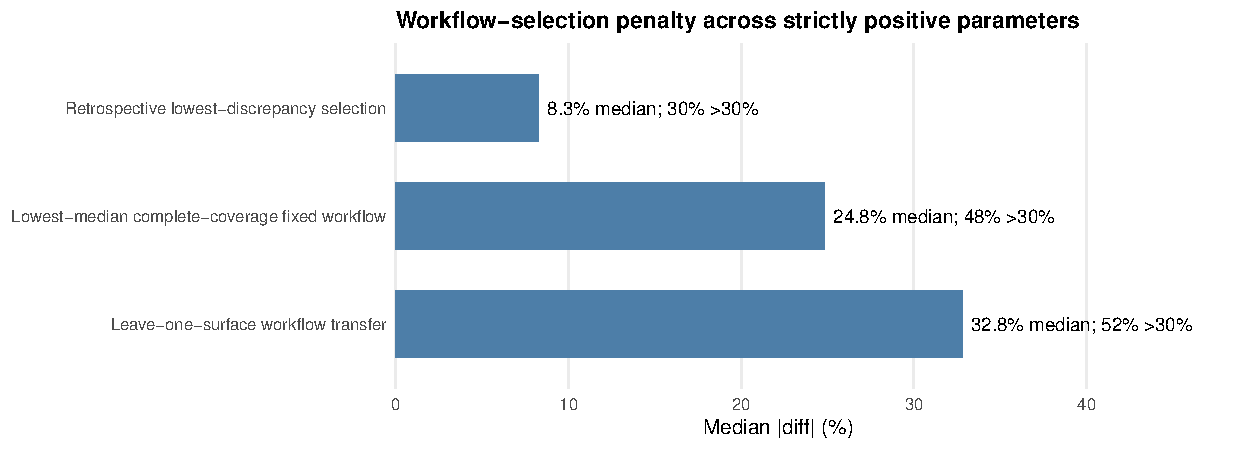
\includegraphics[width=0.92\linewidth]{../plots/workflow_selection_penalty_overview.pdf}
	\caption{Workflow-selection penalty across the seven strictly positive roughness parameters. Bars show the median $|\mathrm{diff}|(\%)$ for retrospective lowest-discrepancy selection, the lowest-median complete-coverage fixed workflow, and leave-one-surface workflow transfer; labels also report the percentage of groups above 30\% discrepancy.}
	\label{fig:workflow_selection_penalty}
\end{figure}

Figure~\ref{fig:global_best_discrepancy_heatmap} summarises the same retrospective lowest-discrepancy benchmark as a process--parameter map. It is derived from the same retrospective workflow-selection logic as Table~\ref{tab:decision_by_param}, but retains the process dimension. It highlights two practically important patterns. First, the retained exported-value $R_{sm}$ comparison remains close to 100\% median discrepancy across all processes even after retrospective workflow selection. Second, amplitude parameters show strong process dependence: rough wire EDM, honing, glass bead blasting, and finish wire EDM generally occupy the low-discrepancy region, whereas rough face turning and rough milling contain several higher-discrepancy cells.

\begin{figure}[H]
	\centering
	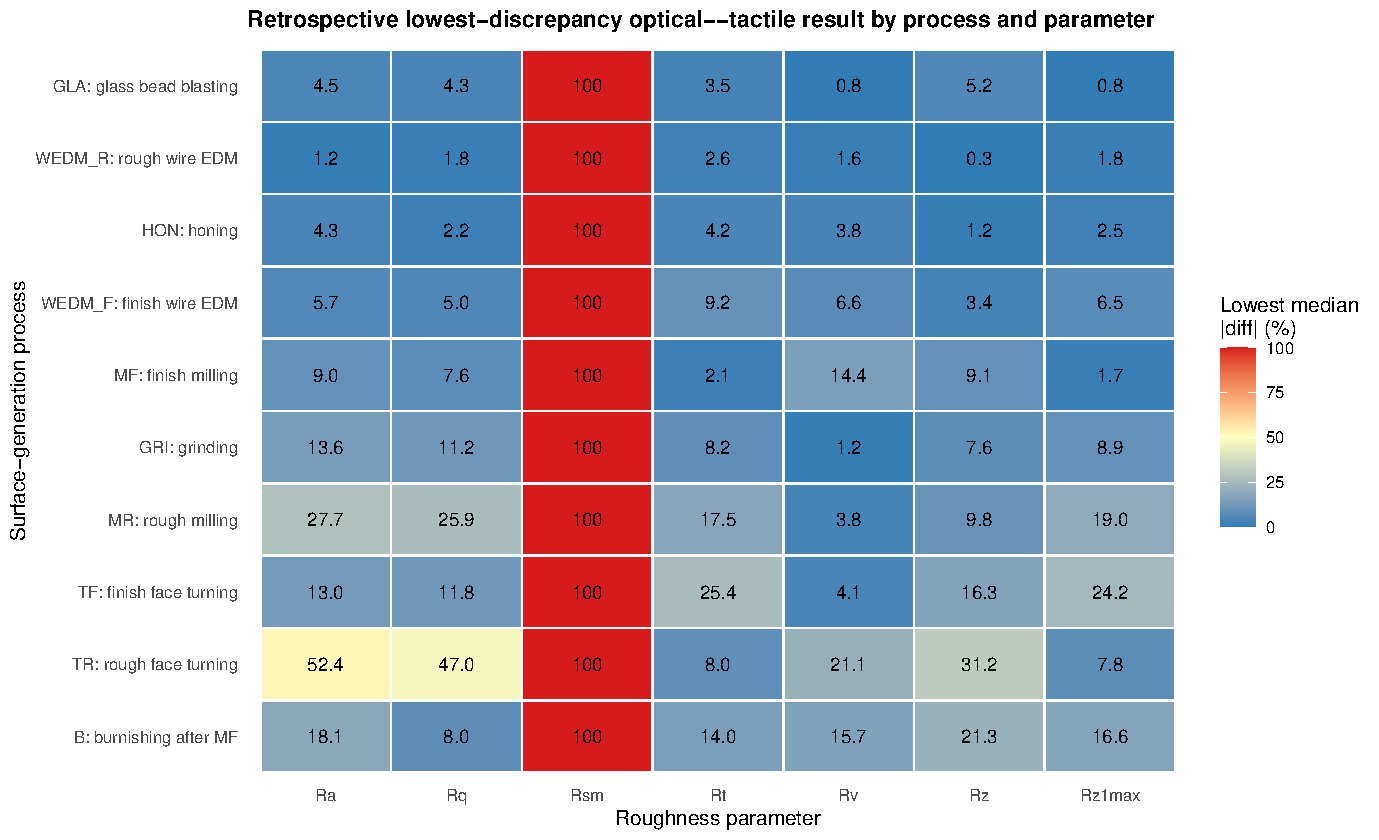
\includegraphics[width=0.98\linewidth]{../plots/global_best_discrepancy_heatmap.pdf}
	\caption{Global process--parameter map of retrospective lowest-discrepancy optical--tactile median discrepancy for the seven strictly positive roughness parameters. Values are median $|\mathrm{diff}|(\%)$ after selecting the lowest-discrepancy available system--illumination pair within each material--process--parameter group; colour scale is capped at 100\% for readability.}
	\label{fig:global_best_discrepancy_heatmap}
\end{figure}

Across the full dataset, interferometry-based measurements (\textit{int}) appear most frequently as the retrospective lowest-discrepancy configuration for most parameters, and red/green illumination bands are most often associated with the lowest-discrepancy median $|\mathrm{diff}|(\%)$ (Table~\ref{tab:decision_by_param}). Process- and material-specific exceptions are also present, with other systems, notably focus variation (\textit{FV}), becoming the most frequent lowest-discrepancy choice in selected strata (Tables~\ref{tab:decision_by_process}--\ref{tab:decision_by_material}). These frequencies describe patterns within the tested archive.

Figure~\ref{fig:effects_by_system} illustrates the main effects of the measurement system on the absolute percentage error using the representative case of $R_a$ on Ti6Al4V after finish milling. Analogous plots for other material--process combinations are included in the supplementary materials.

\begin{figure}[H]
	\centering
	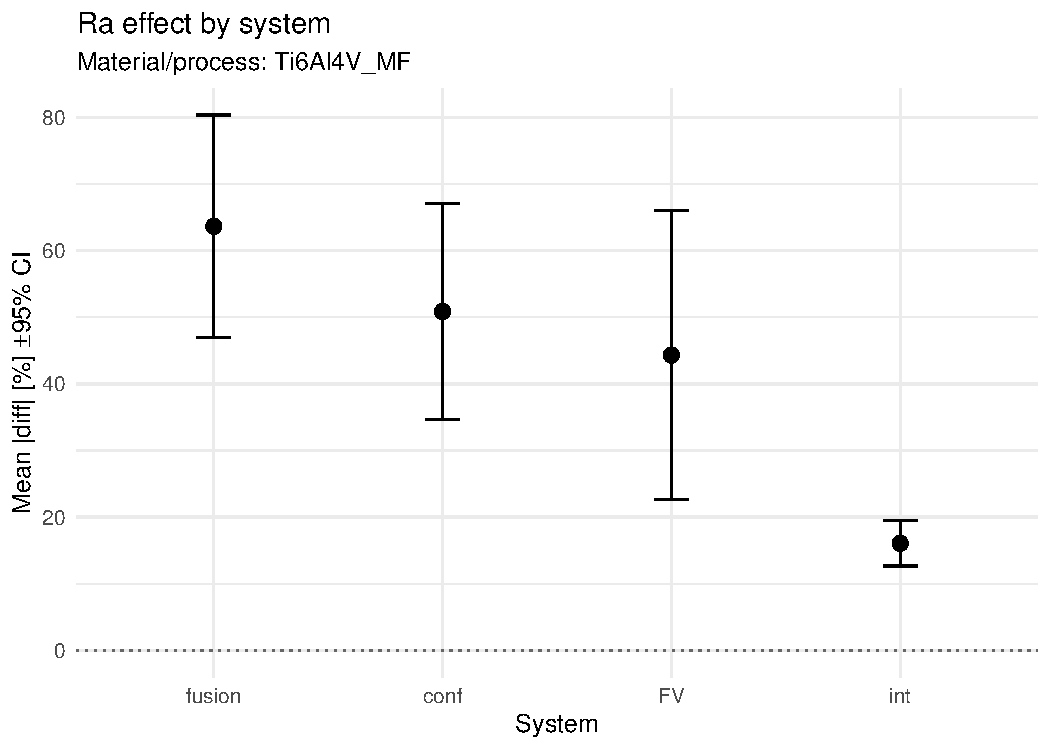
\includegraphics[width=0.9\linewidth]{../plots/ra_abs_ti6al4v_mf_effects_by_system.pdf}
  \caption{Main effects of the measurement system on absolute roughness error $|\mathrm{diff}|(\%)$ for $R_a$ on Ti6Al4V after finish milling}
	\label{fig:effects_by_system}
\end{figure}

\subsection{\texorpdfstring{Representative example: Ti6Al4V after\\finish milling}{Representative example: Ti6Al4V after finish milling}}
To illustrate the system-to-system variability observed across the full dataset, a detailed example is shown for Ti6Al4V after finish milling, which represents a technologically relevant, moderately smooth surface. In the decision summaries, roughly half of all available $R_a$ material--process groups reach $\leq 10\%$ discrepancy after selecting the lowest-discrepancy optical system and colour (Table~\ref{tab:decision_by_param}), while Ti6Al4V is among the more challenging materials in aggregate (Table~\ref{tab:decision_by_material}).

For Ti6Al4V after finish milling, the spread of $|\mathrm{diff}|(\%)$ between systems is particularly clear. Some optical instruments yield errors close to the tactile reference under suitable illumination, whereas other configurations deviate markedly. Optical--tactile discrepancy is reported at the \emph{system+illumination} level.

Figure~\ref{fig:optics_vs_tactile} compares the distributions of $|\mathrm{diff}|(\%)$ for all optical systems against the tactile reference for Ti6Al4V after finish milling, emphasising the contrast between well-performing and outlying configurations.

\begin{figure}[H]
	\centering
	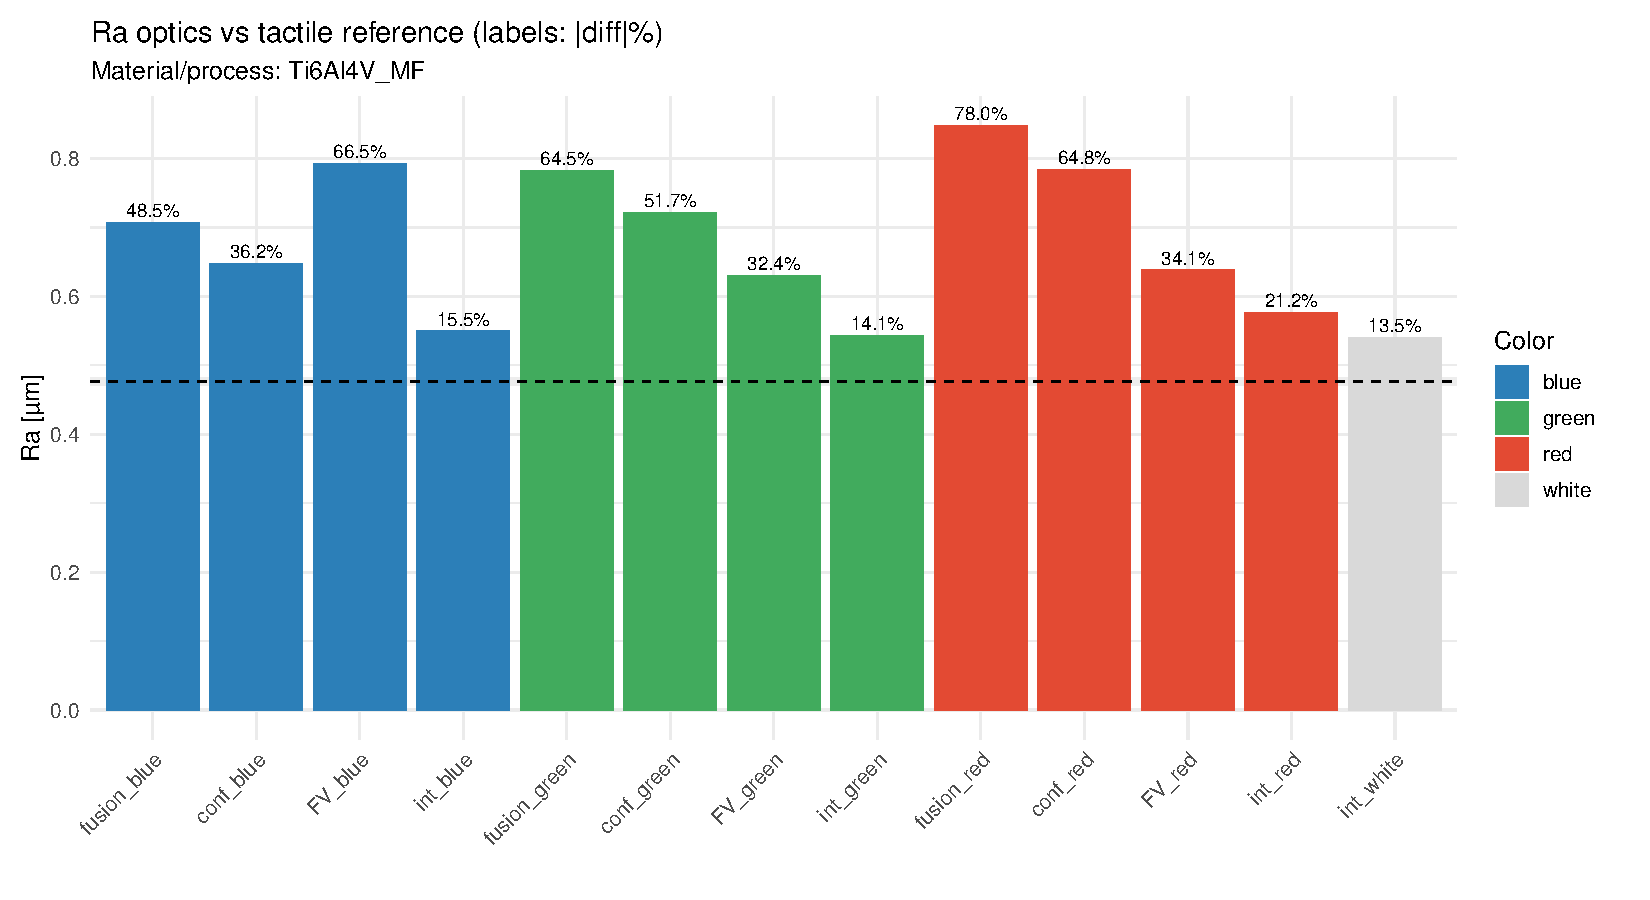
\includegraphics[width=0.9\linewidth]{../plots/ra_abs_ti6al4v_mf_optics_vs_tactile.pdf}
  \caption{Comparison of absolute roughness error $|\mathrm{diff}|(\%)$ for $R_a$ on Ti6Al4V after finish milling obtained from optical systems and the tactile reference}
	\label{fig:optics_vs_tactile}
\end{figure}

\subsection{Influence of illumination wavelength}
Across materials and processes, illumination colour can shift $|\mathrm{diff}|(\%)$ and, in a minority of cases, induces systematic trends with wavelength. In the full set of system-wise regressions across the analysed material--process--parameter groups, statistically significant slopes $\beta_1$ of $|\mathrm{diff}|(\%)$ versus wavelength were observed in 8.9\% of fits (203/2290), indicating wavelength optimisation as an application-specific tuning step rather than a universal correction.
The regressions span many parameter--surface groups and typically rely on only three or four colour levels per fit; individual significant slopes serve as screening evidence. The observed rate is only modestly above the nominal 5\% false-positive rate, so the archive supports selective wavelength effects rather than a broad wavelength law.

Consistent with this, ANOVA effect sizes indicate that the measurement system accounts for substantially more variability in $|\mathrm{diff}|(\%)$ than illumination colour for most groups (median $\eta^2_{\text{system}}=0.651$ vs. median $\eta^2_{\text{color}}=0.106$ across all ANOVA groups, $n=590$; Supplementary Table~S1). Across the same 590 parameter--surface groups, the system effect size exceeds the colour effect size in 497 cases, whereas colour exceeds system in 93. Nevertheless, colour still matters operationally because the lowest-discrepancy configuration for many parameters is tied to a specific illumination band (Table~\ref{tab:decision_by_param}), and these preferences can differ across process and material (Tables~\ref{tab:decision_by_process}--\ref{tab:decision_by_material}).

The full per-group ANOVA outputs (including degrees of freedom, $F$, $p$, and $\eta^2$) are reported in Supplementary Table~S1, and the full set of system-wise wavelength-regression slopes is reported in Supplementary Table~S2. Correlation coefficients were used as a complementary descriptive diagnostic alongside regression; to avoid redundancy, the paper reports regression slopes as the primary summary. Additional system- and colour-wise effect plots supporting follow-up comparisons are provided in the supplementary materials.

Figure~\ref{fig:diff_vs_wavelength} shows an example of the dependence of $|\mathrm{diff}|(\%)$ on illumination wavelength for $R_a$ on Ti6Al4V after finish milling, together with fitted screening lines that illustrate the estimated trend for each optical system.

\begin{figure}[H]
	\centering
	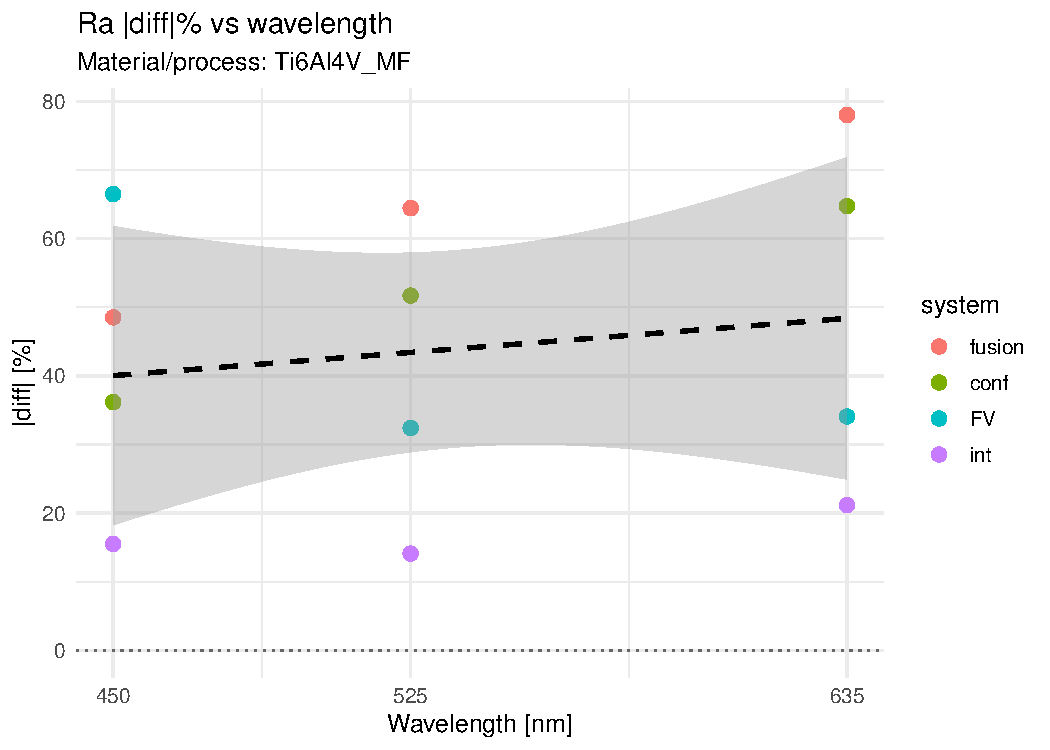
\includegraphics[width=0.9\linewidth]{../plots/ra_abs_ti6al4v_mf_diff_vs_wavelength.pdf}
  \caption{Dependence of absolute roughness error $|\mathrm{diff}|(\%)$ for $R_a$ on Ti6Al4V after finish milling on illumination wavelength for individual optical systems; lines indicate fitted screening trends}
	\label{fig:diff_vs_wavelength}
\end{figure}

\subsection{Technical distance between systems}
The technical distance matrix derived from mean $|\mathrm{diff}|(\%)$ highlights clusters of optical systems that behave similarly across the investigated materials and surface treatments. Systems within the same cluster tend to exhibit comparable error levels and wavelength trends, whereas isolated systems form distinct groups at large distances from the rest. Small distances indicate similar discrepancy patterns within the analysed dataset, separately from matched metrological behaviour, shared traceability, or a common calibration strategy.
As a representative example, Figure~\ref{fig:tech_distance} shows the technical distance matrix for $R_a$ on Ti6Al4V after finish milling. Equivalent matrices for other material--process combinations and parameters are available in the supplementary materials, and they provide a compact complement to the decision tables (Tables~\ref{tab:decision_by_param}--\ref{tab:decision_by_material}) by showing which systems behave similarly \emph{within a given material--process context}.

\begin{figure}[H]
	\centering
	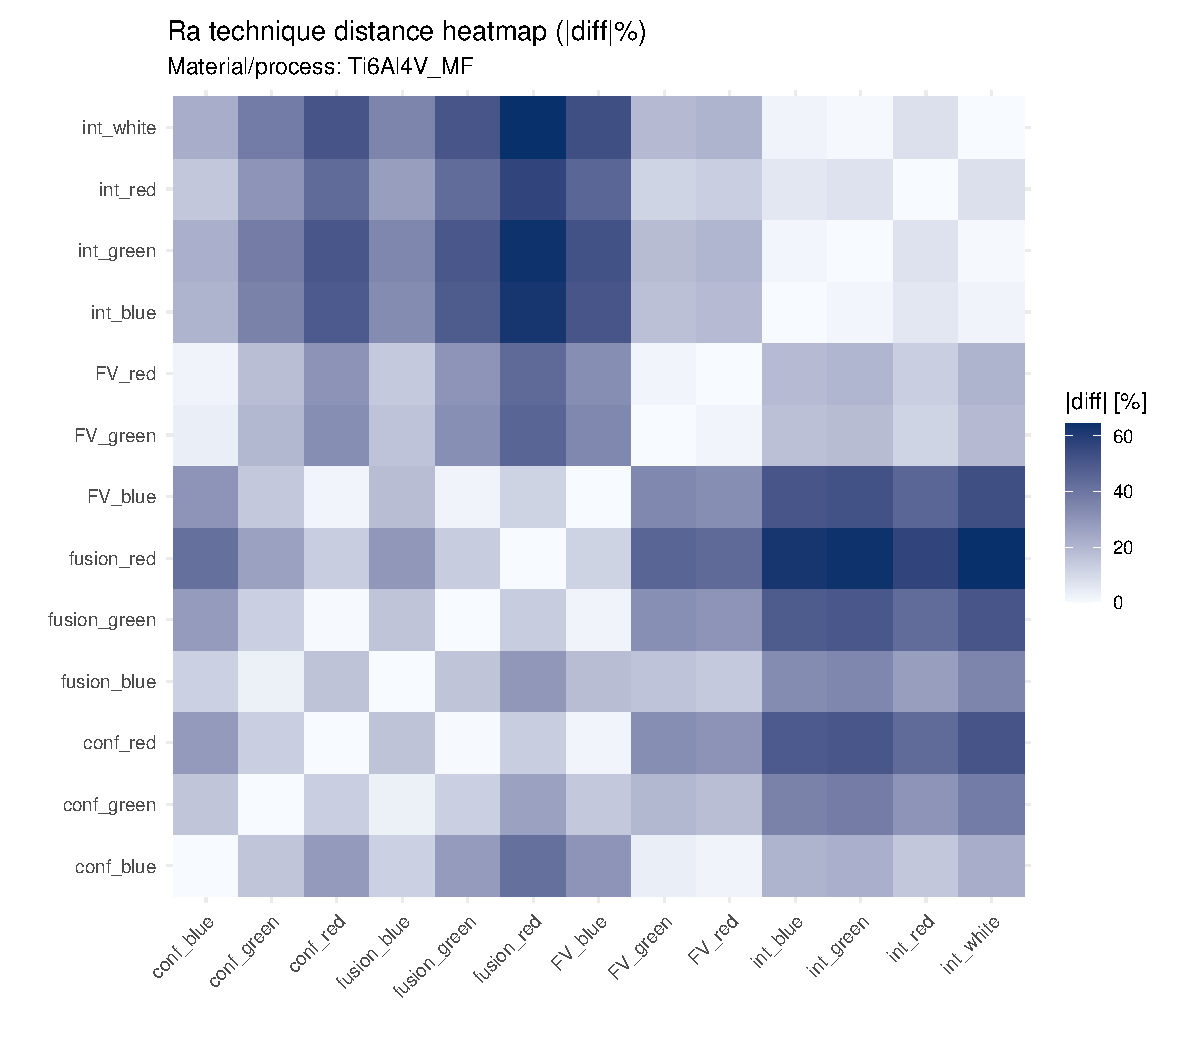
\includegraphics[width=0.9\linewidth]{../plots/ra_abs_ti6al4v_mf_tech_distance_heatmap.pdf}
  \caption{Technical distance matrix between optical and tactile systems for $R_a$ on Ti6Al4V after finish milling, based on mean absolute roughness error $|\mathrm{diff}|(\%)$}
	\label{fig:tech_distance}
\end{figure}

\section{Discussion}\label{sec:discussion}

A multi-material retrospective benchmark of optical workflows against an internal tactile baseline has been presented. Within the archive and its parameter-label comparison frame, three patterns are robust. First, system choice dominates the discrepancy structure across the archive. Second, illumination band matters, but mainly as a secondary, system-specific tuning variable. Third, performance is strongly parameter-dependent: amplitude-type parameters can enter a lower-discrepancy regime under selected configurations, whereas $R_{sm}$ remains difficult.

The stronger transfer of amplitude parameters is physically plausible within the retained comparison frame. Parameters such as $R_t$, $R_v$, $R_z$, and $R_{z1max}$ are mainly governed by height reconstruction, local reflectance, outlier sensitivity, and the vertical response of the optical workflow. By contrast, spacing and shape descriptors depend additionally on lateral sampling, profile extraction, feature recognition, filtering, and the interaction between optical footprint and surface topography. This difference helps explain why some amplitude parameters show useful low-discrepancy candidates, while $R_{sm}$ behaves as a separate harmonisation problem.

The $R_{sm}$ results should be interpreted as a harmonisation-sensitive diagnostic. The near-constant 99.9\% discrepancy in the retained exported values, together with the large tactile/optical ratio, is consistent with a unit-convention mismatch between optical exports (likely in millimetres) and the tactile reference (in micrometres). This interpretation is supported by three lines of evidence: (i)~the near-universal 99.9\% discrepancy across all four optical-system families, all six materials, and all processes (Table~\ref{tab:rsm_diagnostic}), which would be unlikely if the effect were due to random optical measurement error; (ii)~the substantial reduction of discrepancy under $\times 1000$ rescaling, which moves 24 of 59 material--process groups into the $\leq 10\%$ band; and (iii)~the known sensitivity of $R_{sm}$ to the profile-element detection rules specified in ISO~21920-3, which may differ from the internal algorithms of commercial optical instrument software. Direct confirmation would require access to the raw optical and tactile profiles, application of a common profile-element detection and filtering chain, and re-computation of $R_{sm}$ under controlled settings---a study that is proposed as a priority follow-up investigation.

The unit-convention sensitivity affecting $R_{sm}$ does not apply to the amplitude parameters. $R_a$, $R_q$, $R_t$, $R_v$, $R_z$, and $R_{z1max}$ are height parameters reported in micrometres by both tactile and optical instruments across the archive, and spot-checking of selected raw exports confirmed that the retained values use consistent length units. No analogous scaling sensitivity was found for these parameters. From a practical standpoint, the $\times 1000$ analysis indicates that a substantial portion of the optical--tactile $R_{sm}$ discrepancy likely originates from a unit-convention mismatch. If the optical exports indeed report $R_{sm}$ in millimetres, then unit harmonisation alone would bring 24 of 59 material--process groups into the low-discrepancy band. However, the 15 groups that remained above 30\% even after $\times 1000$ rescaling (Table~\ref{tab:rsm_scale_sensitivity}) indicate that genuine measurement differences---related to lateral sampling, profile-element recognition, and the effective optical footprint---persist beyond the unit question. For practitioners, the pragmatic recommendation is to verify and explicitly document the $R_{sm}$ unit convention in all optical roughness exports before comparing with tactile spacing values; where the exported unit cannot be confirmed, $R_{sm}$ should be excluded from optical-substitution claims and treated solely as a diagnostic endpoint.

The decision tables identify the lowest-discrepancy workflow observed within each parameter--surface group and serve as screening tools for follow-up validation. The ANOVA decompositions and wavelength regressions summarise patterns in an unbalanced archive, especially where only three or four illumination levels were available, and provide archive-level screening rather than causal or transferable correction models. Percentage-based $R_{sk}$ summaries are retained in the archive-derived tables as secondary descriptors, separately from the strictly positive parameters.

Percentage normalisation of $R_{sk}$ is intrinsically unstable because tactile baseline values near zero inflate the denominator in Equation~\ref{eq:diff}, producing exaggerated percentage discrepancies even when the absolute difference is modest. For future sign-sensitive parameter comparisons, an alternative reporting metric would be the absolute difference $\Delta_{sk}=O_{sk}-S_{sk}$, possibly normalised by the within-group tactile standard deviation $s_S$, or a rank-correlation-based consistency index that is immune to near-zero baselines. The present archive provides $R_{sk}$ percentage summaries as screening-level secondary descriptors (Supplementary Tables~S1--S5), but decision-oriented interpretation of $R_{sk}$ should await a metric that is stable under near-zero denominators.

Because optical acquisition settings---objective numerical aperture, field of view, lateral sampling interval, vertical scan range, and form-removal operator---were not retained uniformly across the archive, the benchmark cannot separate discrepancies originating from the optical measurement principle from those arising from operator-selected processing parameters. The same optical sensor can produce substantially different roughness outputs under different filtering and form-removal choices~\cite{ISO16610-21-2011,Boedecker2010}. Consequently, the workflow rankings characterise the specific instrument--settings--processing chain represented in the archive rather than inherent properties of the optical technique. Prospective validation must control and document these settings.

Optical repeat measurements were retained less consistently than tactile repeats. Where optical replication exists in the archive, it is limited to a small subset of parameter--surface groups and does not permit a formal between-workflow repeatability comparison. A limited sensitivity check on the groups with partial optical replication indicated that optical repeatability standard deviations are generally smaller than the between-workflow discrepancy medians reported here, but this check is archive-limited and cannot substitute for a designed gauge R\&R study.

The fixed-configuration sensitivity analysis separates archive screening from preselected-workflow use. In the screening view, the retrospective lowest-discrepancy summaries identify promising follow-up candidates. In the fixed-workflow view, one optical setup is evaluated before measurement across all available groups. The gap between these views is substantial: the lowest-median complete-coverage fixed workflow has a median discrepancy of 24.8\%, whereas several amplitude parameters achieve medians below 10\% only after the workflow is allowed to vary by parameter--surface group. The leave-one-surface workflow-transfer check strengthens the same point: even when the workflow is selected from other material--process groups of the same parameter, the held-out median discrepancy is 32.8\%, and 52\% of held-out groups remain above 30\%. The transfer penalty is not uniform across the benchmark. Amplitude parameters show smaller transfer penalties for C45 steel across machining processes and for ground surfaces generally, suggesting that these material--process classes share sufficient textural similarity for a workflow learned on one class to transfer usefully to another. $R_a$ and $R_q$ show systematically larger transfer penalties than $R_t$ and $R_z$, indicating that the arithmetic-average roughness is more sensitive to the specific material--process context than the peak-to-valley extremes. Cross-material transfer penalties are systematically larger than cross-process transfer penalties within the same material, consistent with the dominant role of material optical properties. For a laboratory that must preselect one optical workflow, discrepancies of this order remain expected unless a narrower material--process range is validated prospectively. Optical workflow selection is therefore part of the metrological decision, and the manuscript decision bands are most appropriately read as validation priorities rather than as direct specification limits.

A practical selection dilemma arises when a single optical system performs well for one roughness parameter but poorly for another on the same surface. The decision tables show that interferometry-based configurations tend to provide the most consistent low-discrepancy performance across the amplitude parameters, whereas confocal systems perform well for $R_z$ and $R_{z1max}$ on materials with moderate reflectance. Where a single system must serve multiple parameters, the fixed-workflow analysis provides the relevant performance baseline: interferometry with green illumination achieved median discrepancy 24.8\% with complete coverage (Table~\ref{tab:fixed_workflow_sensitivity}). Practitioners who need lower discrepancies for a specific parameter can consult the per-parameter decision tables to identify the most promising system--illumination candidate for prospective, single-parameter validation.

From a technological perspective, the archive supports workflow triage rather than workflow substitution. For manufacturing surfaces similar to those represented in the archive, amplitude-type descriptors such as $R_t$, $R_v$, $R_z$, $R_{z1max}$, and in many cases $R_a$ and $R_q$, are the more plausible candidates for rapid optical screening after workflow-specific validation. In contrast, exported $R_{sm}$ should be treated as a spacing- and scale-sensitive diagnostic, especially after surface treatments or processes that alter texture periodicity, local slope, reflectance, or missing-data behaviour. The practical implementation lesson is that the optical system and processing chain should be selected and validated first for the relevant material--process--parameter group, with illumination colour or wavelength treated as a secondary tuning variable. For treated, highly reflective, irregular, steep, or otherwise optically difficult surfaces, tactile confirmation remains the more defensible route until a workflow-specific validation has been performed. For laboratories using multiple instruments, the technical distance maps provide an operational summary of which workflows behave similarly within a given material--process context, separately from shared calibration or metrological equivalence.

A supplementary mapping of the observed discrepancy ranges to ISO~21920-3 profile tolerance grades provides a familiar metrological reference frame. ISO~21920-3 defines tolerance grades TG1--TG6 for profile parameters, with the finest grade (TG1) requiring agreement within approximately $\pm 5\%$ of nominal and the coarsest grade (TG6) within approximately $\pm 25\%$, depending on the parameter and the nominal range. The retrospective lowest-discrepancy medians of 4.8--6.6\% for $R_t$, $R_v$, $R_z$, and $R_{z1max}$ would correspond approximately to TG2--TG3, whereas the median fixed-workflow discrepancy of 24.8\% corresponds to TG6, the coarsest tolerance class. This mapping is illustrative rather than normative: ISO tolerance grades apply to conformance testing under controlled conditions with a documented measurement process, not to retrospective benchmarking. It is presented here to translate the discrepancy percentages into a terminology familiar to manufacturing metrologists.

For stronger tactile--optical equivalence claims, a prospective validation study designed to establish workflow-specific optical--tactile agreement would require: (i)~a predefined material--process--parameter scope with specified ISO GPS filtering and evaluation settings; (ii)~at least 15--20 independent specimens per material--process group, each measured under repeatability conditions on both tactile and optical instruments; (iii)~within-instrument repeatability characterised through repeated measurements ($n \geq 10$) on the same specimen; (iv)~between-instrument reproducibility assessed through a designed gauge R\&R study; (v)~a combined uncertainty budget following GUM principles~\cite{JCGM100-2008}, incorporating tactile calibration uncertainty, optical vertical and lateral calibration, form-removal and filtering contributions, environmental effects, and operator variability; (vi)~pre-specified acceptance criteria expressed as maximum permissible error or as an equivalence margin derived from the intended application tolerance. System and illumination settings would be fixed a priori, or selected in a separate development phase, rather than retrospectively optimised on the reporting dataset. The present benchmark serves as a screening tool to select the most promising parameter--material--process combinations for such a resource-intensive validation.

\subsection{Interpretive scope}
Several features define the scope of the present conclusions. The study compares exported roughness parameters in a harmonised comparison space defined by matched material--process identifiers and same-named parameter labels. The reported discrepancies characterise workflow-level discrepancy within this comparison space. The tactile mean is an internal baseline derived from $n=20$ repeats with an available repeatability descriptor ($s_S$, $u_S$). The tactile repeatability analysis indicates that the random variability of tactile measurements is usually smaller than the observed optical--tactile discrepancies, while unmodelled tactile bias or calibration effects may still shift individual discrepancies. Optical repeat measurements were retained less consistently than tactile repeats, so the optical side of the benchmark is an archived-output comparison. The decision tables are retrospective, with the lowest-discrepancy system+colour selected after observing the data; the fixed-configuration and leave-one-surface transfer analyses quantify this selection effect from complementary perspectives. Bootstrap intervals in Supplementary Table~S5 describe stability of the archive-level median summaries, not formal uncertainty of future optical use. Wavelength regressions and the descriptive summaries in Supplementary Tables~S2--S3 are often based on only three or four colour levels per system and provide screening trends. Raw profiles, common filtering settings, complete optical instrument metadata, detailed process settings, and a combined tactile--optical uncertainty model were retained unevenly across the archive. Percentage-based $R_{sk}$ summaries are intrinsically unstable near zero and are retained as secondary screens.

\section{Conclusions}

Within this scope, the main findings of the multi-material benchmark can be summarised as follows:
\begin{itemize}
	\item \textbf{System choice is the primary workflow driver.} Across the ANOVA screens, the measurement system has a much larger effect size than illumination colour in most groups (median $\eta^2_{\mathrm{system}}=0.651$ versus $\eta^2_{\mathrm{colour}}=0.106$), while wavelength/colour behaviour remains a system-specific tuning issue rather than a universal correction (Supplementary Tables~S1--S2).
	\item \textbf{Parameter dependence is substantial.} Retrospective lowest-discrepancy medians differ sharply across the strictly positive parameters: amplitude-type measures such as $R_t$, $R_v$, $R_z$, and $R_{z1max}$ achieve medians of 4.8--6.6\%, $R_a$ and $R_q$ remain below 10\%, and retained exported-value $R_{sm}$ remains a harmonisation-sensitive spacing diagnostic (Tables~\ref{tab:decision_by_param}--\ref{tab:rsm_scale_sensitivity}).
	\item \textbf{Fixed and transferred workflow choices carry a clear penalty.} The lowest-median complete-coverage fixed workflow has median discrepancy 24.8\%, while leave-one-surface workflow transfer yields a held-out median of 32.8\%, with 52\% of held-out groups above 30\% (Table~\ref{tab:fixed_workflow_sensitivity}, Table~\ref{tab:workflow_transfer}, and Figure~\ref{fig:workflow_selection_penalty}).
	\item \textbf{Tactile Type A uncertainty is low relative to most optical discrepancies.} Across all $472$ parameter--surface groups, the tactile baseline is based on $n=20$ repeats. For the seven strictly positive parameters, the median relative Type A standard uncertainty of the tactile mean is $1.45\%$ (Q1--Q3: 0.85--2.44\%), supporting its use as an internal repeatability benchmark, although not replacing a full uncertainty budget.
	\item \textbf{The main output is a benchmark for follow-up selection.} The decision summaries identify candidate optical workflows for prospective validation in specific parameter--surface groups. They prioritise follow-up experiments rather than establishing a universal fixed optical setup or formal tactile/optical equivalence.
\end{itemize}

Overall, the benchmark identifies where optical roughness workflows are plausible candidates for prospective validation and where tactile confirmation remains the more defensible route. Its main value is not an equivalence claim, but a reproducible decision map separating local low-discrepancy matches from fixed-workflow and held-out transfer performance.

\section*{Supplementary materials}
The following supporting information is available online at the journal website:
\begin{itemize}
	\item \textbf{Supplementary S1}: additional tables and figures extending the Results. The material includes (i) two-way ANOVA main effects and $\eta^2$ effect sizes for the factors system and colour (Supplementary Table~S1), (ii) system-wise slopes of $|\mathrm{diff}|(\%)$ versus illumination wavelength (Supplementary Table~S2), (iii) descriptive statistics by system (Supplementary Table~S3), (iv) parameter-wise internal tactile repeatability summaries (Supplementary Table~S4), and (v) bootstrap percentile intervals for aggregate retrospective lowest-discrepancy medians (Supplementary Table~S5), together with representative plots for selected material--process combinations. The supplementary tables are generated from the same archived output files as the manuscript tables, and the generation script is included in the public repository.
\end{itemize}

\section*{Data availability}
The R/Python analysis scripts, configuration files, manuscript and supplement sources, generated CSV outputs, generated tables, and generated figures supporting the findings are provided as submission reproducibility materials. Public repository and archive identifiers are supplied separately for editorial handling and can be inserted in the final version according to journal anonymisation policy. Raw \texttt{.sur} surface files are excluded from the public package as original instrument exports with size and transfer constraints; the derived CSV outputs needed to reproduce the manuscript tables, fixed-workflow sensitivity analysis, workflow-transfer check, global heatmap, selection-penalty figure, and supplementary tables are included. The excluded raw \texttt{.sur} files are available from the authors on reasonable request, subject to data-transfer constraints.

% References are supplied via BibTeX; set style as needed for the target journal.
%\bibliographystyle{elsarticle-num}
\bibliographystyle{unsrt}
\bibliography{bibliography}

\end{document}